% 1. fact check claim that other brain parcellation studies use
%    Pearson's correlation (not absolute value) as edge weights
%#######################################################################

Paragraph 1: Write here what would happen in the ideal world

Paragraph 2: Write here why we cannot reach this ideal easily

Paragraph 3: Write here what we do instead to overcome this problem

\section{fMRI Background}

{\color{blue}

Functional magnetic resonance imaging or functional MRI (fMRI) is a
functional neuroimaging procedure using MRI technology that measures
brain activity by detecting changes associated with blood flow.
When an area of the brain is in use, blood flow to that region also
increases. The primary form of fMRI uses the blood-oxygen-level
dependent (BOLD) contrast. The fMRI concept builds on the earlier MRI
scanning technology and the discovery of properties of oxygen-rich
blood. 
The basis of MRI revolves around changing the magnetic moment of proton
in hydrogen atoms abundantly found in the human body. MRI brain scans
use a strong, permanent, static magnetic field to align nuclei in the
brain region being studied. Another magnetic field, the gradient field,
is then applied to spatially locate different nuclei.

Finally, a radiofrequency (RF) pulse is played to kick the nuclei to
higher magnetization levels, with the effect now depending on where
they are located. When the RF field is removed, the nuclei go back to
their original states, and the energy they emit is measured with a coil
to recreate the positions of the nuclei. MRI thus provides a static
structural view of brain matter. The central thrust behind fMRI was to
extend MRI to capture functional changes in the brain caused by
neuronal activity. Differences in magnetic properties between arterial
(oxygen-rich) and venous (oxygen-poor) blood provided this link.

The fMRI machine records the relative change detected within a time
frame (typically 2 seconds) in magnetization as a 3-dimensional image.
The 3-dimensionsal image it provides is built up in units called
voxels. Each one represents a tidy cube of brain tissue -- a 3-D image
building block analogous to the 2-D pixel of computers screens,
televisions or digital cameras. When visualized on a monitor, typically
each intensity level is encoded as a varying shade of gray. \{Probably
good to include an image of the ``typical" fMRI scan\}

Each voxel can represent a million or so brain cells. As measurements
are made over time (for example, over 10 minutes), the neuroscietist
collects multiple 3-dimensional images in the form of a time series. 

\{This information was primarily taken from wiki,
\url{https://www.youtube.com/watch?v=djAxjtN\_7VE},
\url{http://science.howstuffworks.com/mri.htm} and
\url{http://www.howequipmentworks.com/mri\_basics/}.\}
}

\section{Parcellation Background}

{\color{red} talk about AAL and do the literature review here.}

Functional parcellation of the human brain can be defined as the problem
of partitioning the voxels into $k$ disjoint connected components with
the goal that the voxels within each component are, in a rough sense,
\"similar\" to each other and voxels in different components are less
\"similar\". Such similarity has been defined in a multitude of ways in
the literature [see lit review section ...]. For this project thus far I
have taken similarity between voxels to mean statistical dependence.

\section{Overall Strategy}
{\color{red}
Let's move this stuff about correlation to the beginning of the next
chapter about energy statistics. For now, it's good enough to say in one paragraph that we'll use some nonlinear dependency in our procedure or
something (high level summary)}

To measure dependence, statisticians have traditionally used the Pearson
correlation coefficient, in addition to the rank-based Kendall tau and
Spearman rho. These statistics work well when the underlying
relationship between the two random variables is linear, in the case of
Pearson, or can be linear after a monotonic transformation, in the case
of Kendall and Spearman. Due to their restrictions, these correlation
coefficients will fail to capture many kinds of dependency
relationships. The figure below illustrates several instances of pairs
of random variables whose depencency structure is not detected by the
three correlation coefficients.

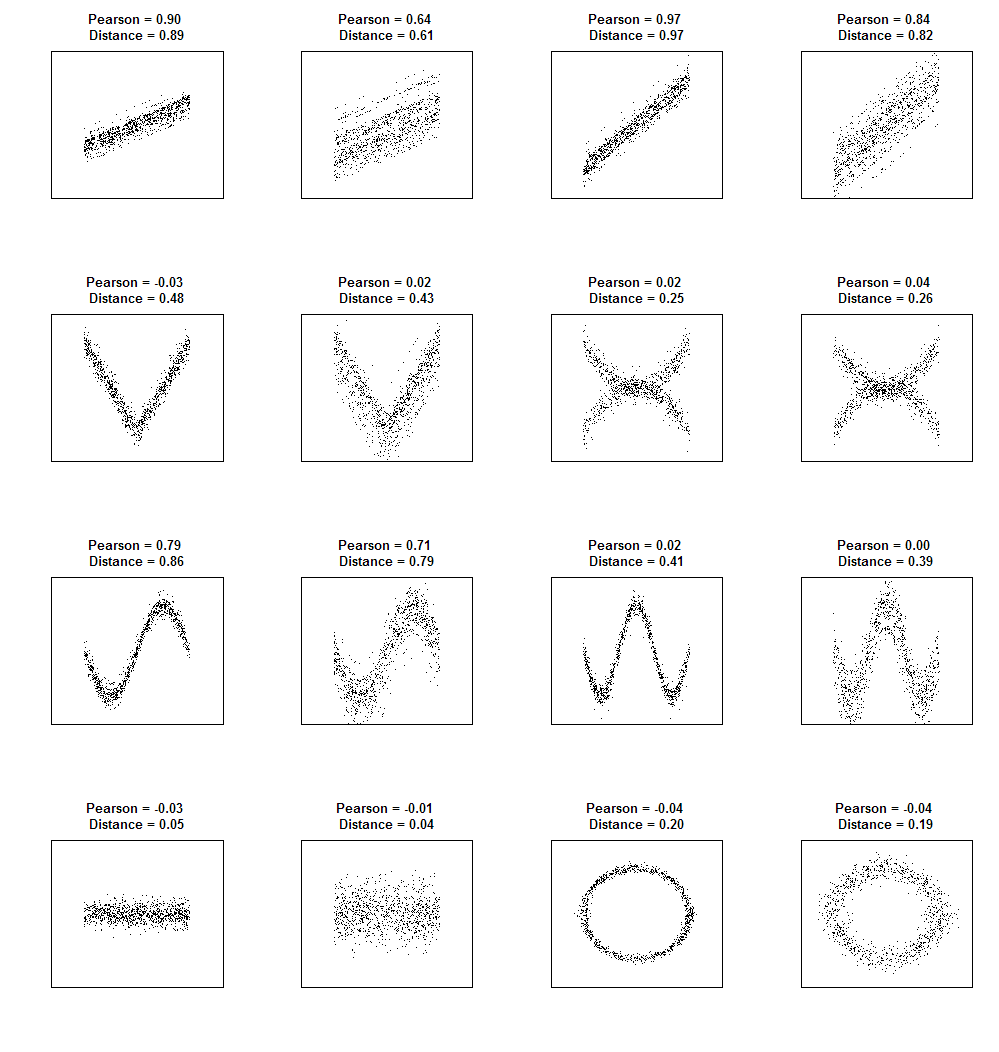
\includegraphics[scale = 0.8]{figs/1_nonlinear_depend.png}

Non-linear dependency relationships also exist in the ABIDE 50002 fMRI
data. The scatterplots below show time samples of spatially adjacent
voxels. These instances were found by searching for the maximum
difference in rank of energy distance correlation and the coefficient
of determination, or Pearson squared.

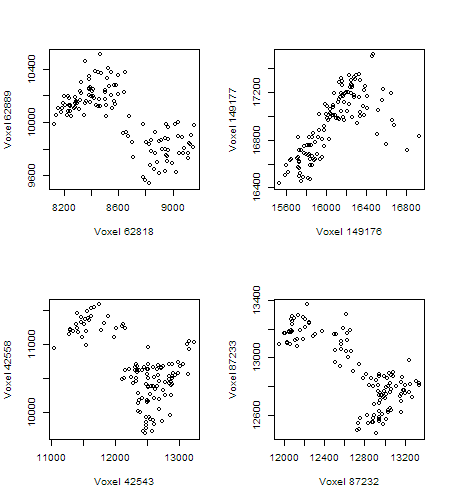
\includegraphics[scale = 0.7]{figs/1_nonlinear_ABIDE_50002.png}

Many studies on functional parcellation (Craddock 2012; Bellec 2006;
Heller 2006) use Pearson's coefficient as the similarity measure between
nearby voxels. Apart from underestimating the important of non-linear
relationships, this method also distinguishes positive, upward-sloping
correlation from negative. As a result in many of the edges between
different parcels, the corresponding voxels would be strongly dependent
with negative correlation.


\section{About the Data}
{\color{blue}

Autism spectrum disorders (ASD) represent a formidable challenge for
psychiatry and neuroscience because of their high prevalence, lifelong
nature, complexity and substantial heterogeneity. Roughly 1\% of
children worldwide are diagnosed with ASD \cite{centers2010autism}.
We approach the parcellation problem by using the Autism Brain Imaging
Data Exchange (ABIDE) -- a consortium aggregating and openly sharing
1112 existing resting-state functional magnetic resonance imaging
(R-fMRI) data sets with corresponding structural MRI and phenotypic
information from 539 individuals with ASDs and 573 age-matched typical
controls (TCs; 7–64 years).

For simplicity in this thesis, we focus on
\{NUMBER OF SUBJECTS YOU'RE ACTUALLY USING\}
scanned at the University of Pittsburgh School of Medicine.
These autistic subjects included individuals from 7 to 35 years of age,
with a well-characterized Autistic Disorder. The Autism Diagnostic
Interview-Revised \cite{lord1994autism} and the Autism Diagnostic
Observation Schedule-General \cite{lord2000autism}, as well as expert
clinical opinion, were used to diagnose autism. Typical controls were
healthy individuals, with no history of head trauma, birth
complications, seizures, or psychiatric disorder. TC matched
individually to the participants with autism on age (within 1.5 y in
children, 3.5 y in adults), full-scale IQ (within 12 points) and gender.
Individuals with Autistic Disorder were referred from the Center for
Excellence in Autism Research (CEFAR) and the Autism Center of
Excellence (ACE). TC were recruited from previous studies at the LNCD or
by fliers and announcements.
\{If you want to know, I got this information from
\url{http://fcon_1000.projects.nitrc.org/indi/abide/}.
You probably can include this url directly or something.\}

In order to register each subject's brain to a common brain space, we
use the Montreal Neurological Institute's standardized brain
\cite{evans19933d,collins1994automatic}.
The MNI wanted to define a brain that is more representative of the
population. They created a new template that was approximately matched
to the Talairach brain in a two-stage procedure. First, they took 241
normal MRI scans, and manually defined various landmarks, in order to
identify a line very similar to the AC-PC line, and the edges of the
brain. Each brain was scaled to match the landmarks to equivalent
positions on the Talairach atlas. They then took 305 normal MRI scans
(all right handed, 239 M, 66 F, age 23.4 +/- 4.1), and used an
automated 9 parameter linear algorithm to match the brains to the
average of the 241 brains that had been matched to the Talairach atlas.
From this they generated an average of 305 brain scans thus transformed
- the MNI305. The current standard MNI template is the ICBM152, which
is the average of 152 normal MRI scans  that have been matched to the
MNI305 using a 9 parameter affine transform. The International
Consortium for Brain Mapping adopted this, the MNI152, as their
standard template, and this is the template we will be using. We use
the unsymmetrical MRI scan from MNI152 corresponding to voxels
corresponding to cubes with an edge-length of 2 millimeters. This
MNI152 template includes \{WHAT ARE THE DIMENSIONS? I'll look this up
lol.\}.

We preprocessed the raw data from ABIDE using the Configurable Pipeline
for the Analysis of Connectomes (C-PAC) alpha version 0.3.9. C-PAC is
an open-source software pipeline for automated preprocessing and
analysis of resting-state fMRI data. The image preprocessing steps
included slice-timing and motion correction based on the Friston Model,
nuisance signal regression (including 5 CompCorr signals, the
cerebrospinal fluid (CSF), motion and the global, linear, and quadratic
signals) and temporal filtering (0.001-0.08Hz). The derived R-fMRI
measures were normalized to Montreal Neurological Institute (MNI152)
stereostatic space (2mm$^3$ isotropic) with linear regressions and
spatially smoothed (applied FWHM = 6mm).

We then converted the 4-dimensional fMRI data (i.e., a 3-dimensional
image varying with time) in a 2-dimensional matrix whereby each column
represents a different voxel and each row represents a different sample
from a different time. Since C-PAC removed most autocorrelations in the
data, we can reasonably treat each observation (i.e, each row) as drawn
from the same unknown distribution.
}

In this investigation, all parcellation and validation procedures were
conducted on the ABIDE 50002 fMRI data set. This data set contains
233305 voxels and 124 time samples. Spatial information is encoded as a
graph; each voxel is represented by a vertex, and each vertex has up to
6 edges connecting the voxel to its cubically adjacent neighbors. The
weights on the edges are sample energy distance correlations between the
two connected voxels (Szekely 2013).

\section{Notation}
{\color{red}If you don't have any, you can omit this section :p}

\section{Chapter Summaries}
{\color{red}Put the last part of what was currently in your abstract
here.}

